\documentclass[12pt]{article}

% \usepackage[default]{sourcecodepro}
% \usepackage[T1]{fontenc}

\usepackage{amsfonts, lipsum}
\usepackage{amsmath,amssymb, amscd,amsbsy, bbm, amsthm, enumerate}
\usepackage{mdframed, titlesec, setspace,verbatim, multicol}
\usepackage[top=1in, bottom=1in, left=.45in, right=.45in]{geometry}
\usepackage[unicode]{hyperref}
\usepackage{tikz, pgfplots, xcolor, fancyhdr}
\usepackage{graphicx, caption, subcaption}
\usepackage{stmaryrd}

\setlength{\parindent}{0pt}
\setlength{\textheight}{9in}

%%% Header and Footer Info
\pagestyle{fancy}
% \fancyhead[L]{{\large CSE431 Assignment 4}}
% \fancyhead[C]{}
% \fancyhead[R]{Name: Bradley Bauer}
\fancyhead[L]{\large CSE 431 Assignment 4 }
\fancyhead[C]{}
\fancyhead[R]{\large Question 4}

\theoremstyle{definition}

%%% These are some shortcuts that are handy
\def\real{{\mathbb R}}
\def\Natural{\mathbb{N}}
\def\dx{\textnormal{dx}}
\def\dy{\textnormal{dy}}
\def\dz{\textnormal{dz}}
\def\dt{\textnormal{dt}}
\def\ds{\textnormal{ds}}
\def\dw{\textnormal{dw}}
\def\Re{\textnormal{Re}}
\def\Im{\textnormal{Im}}
\def\exp{\textnormal{exp}}
\def\interior{\textnormal{interior}}
\def\al{\alpha}
\def\del{\delta}
\def\Del{\Delta}
\def\gam{\gamma}
\def\Gam{\Gamma}
\def\Om{\Omega}
\def\ep{\varepsilon}
\def\lam{\lambda}
\def\rational{{\mathbb Q}}
\def\integer{{\mathbb Z}}
\def\Q{{\mathbb Q}}
\def\Z{{\mathbb Z}}
\def\N{{\mathbb N}}
\def\R{{\mathbb R}}
\def\grad{\nabla}
\def\C{\mathcal C}
\def\P{\mathcal P}
\def\T{\mathcal T}
\def\I{\mathcal I}
\newcommand{\abs}[1]{\left| #1 \right|}
\newcommand{\inner}[1]{\langle #1 \rangle}
\newcommand{\norm}[1]{\left\lVert#1\right\rVert}
\newcommand{\spanvect}{\textnormal{span}}
\newcommand{\union}{\cup}
\newcommand{\Union}{\bigcup}
\def\intersect{\cap}
\def\Intersect{\bigcap}

\newtheorem{innercustomthm}{}
\newenvironment{question}[1]
  {\renewcommand\theinnercustomthm{#1}\innercustomthm}
  {\endinnercustomthm}

\begin{document}

\begin{question}{Hypothesis}
  I expect the array to perform better than the binary tree for inputs of size less than 4096 (page size).
\end{question}

\begin{question}{Methods}
    The experiment is ran on Ubuntu 19.04. GCC version is 8.3 and python version is 3.7.3.
    Also, matplotlib, pandas, and numpy are dependencies of plot.py\\\\
    To run the experiment, first compile
    $$\text{g++ -fconcepts -std=c++2a -O3 code.cpp}$$
    Then execute $$\text{./a.out}$$
    which may take a few minutes to run.
    To plot the results use
    $$\text{python3 plot.py}$$
    The program compares sorted array and binary tree insertion performance for various input sizes n in the range [0, 1e4].
    For each input size n, the program inserts n uniform random integers into a sorted array and into a binary tree.
    The total time taken for inserting n elements into each data structure is recorded.
\end{question}

\newpage
\begin{question}{Results}
$\\$
\begin{figure}[h]
  \centering
  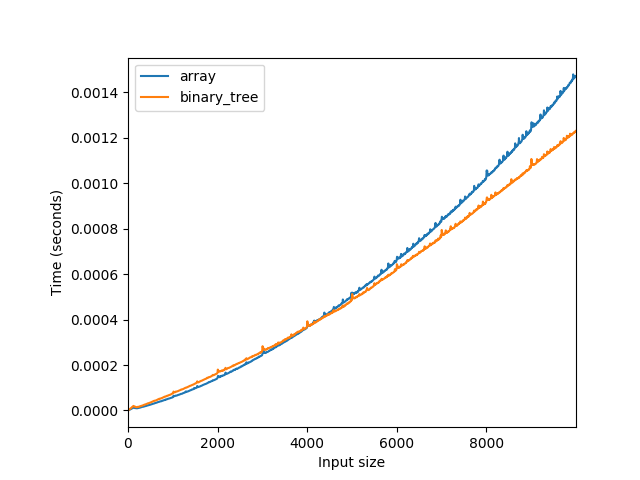
\includegraphics[width=\textwidth]{Figure_2.png}
  \caption{}
  \label{fig:boat2}
\end{figure}
\begin{figure}[h]
  \centering
  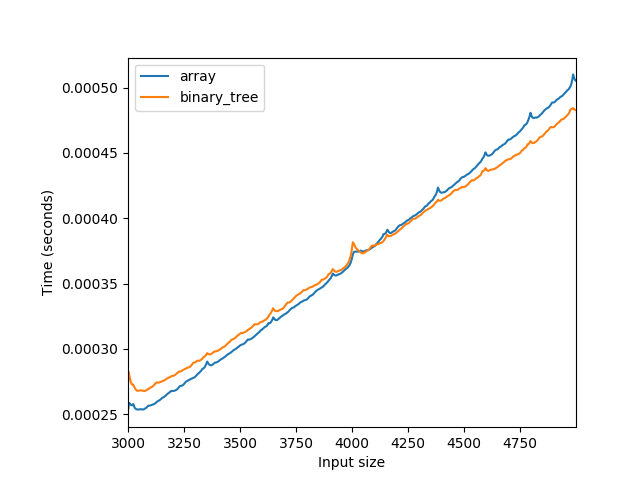
\includegraphics[width=\textwidth]{Figure_4.png}
  \caption{}
  \label{fig:boat2}
\end{figure}

Figure 1 shows average time to insert n elements vs n.
\newpage
Figure 2 a zoomed in view of the previous plot to clearly show the intersection point.

\end{question}

\begin{question}{Discussion}
  Figure 2 shows that the intersection point is roughly 4096 which is the page size on my machine.
\end{question}

\begin{question}{Conclusion}
  The sorted array is a faster datastructure for maintaining relatively small sorted lists.
\end{question}

\end{document}
